
\begin{lemma}{7.2.349}\label{lem:7-2-349}
存在滤过 $A_{n',K'}$ 代数
\[
C_2([0,1]^2\times L'_1,
(\lambda'_0,\lambda'_1)),
\]
它是 $[0,1]^2\times
C(L'_1,(\lambda'_0,\lambda'_1))$
的 $A_{n',K'}$ 类模型；
还存在滤过 $A_{n',K'}$ 同态
\[
\widetilde{\mathfrak H}_2\colon
C(L'_0,\lambda'_0)
\longrightarrow
C_2([0,1]^2\times L'_1,
(\lambda'_0,\lambda'_1)),
\]
使得
\begin{equation}
\operatorname{Eval}_{s=s_0}\circ
\widetilde{\mathfrak H}_2
=\operatorname{Incl}_r\circ\mathfrak f^{\phi'},
\tag{7.2.350}\label{eq:7-2-350}
\end{equation}
且下列图式~\ref{diag:7-2-33} 交换：

\par\medskip\noindent\begin{minipage}{\textwidth}
\centering
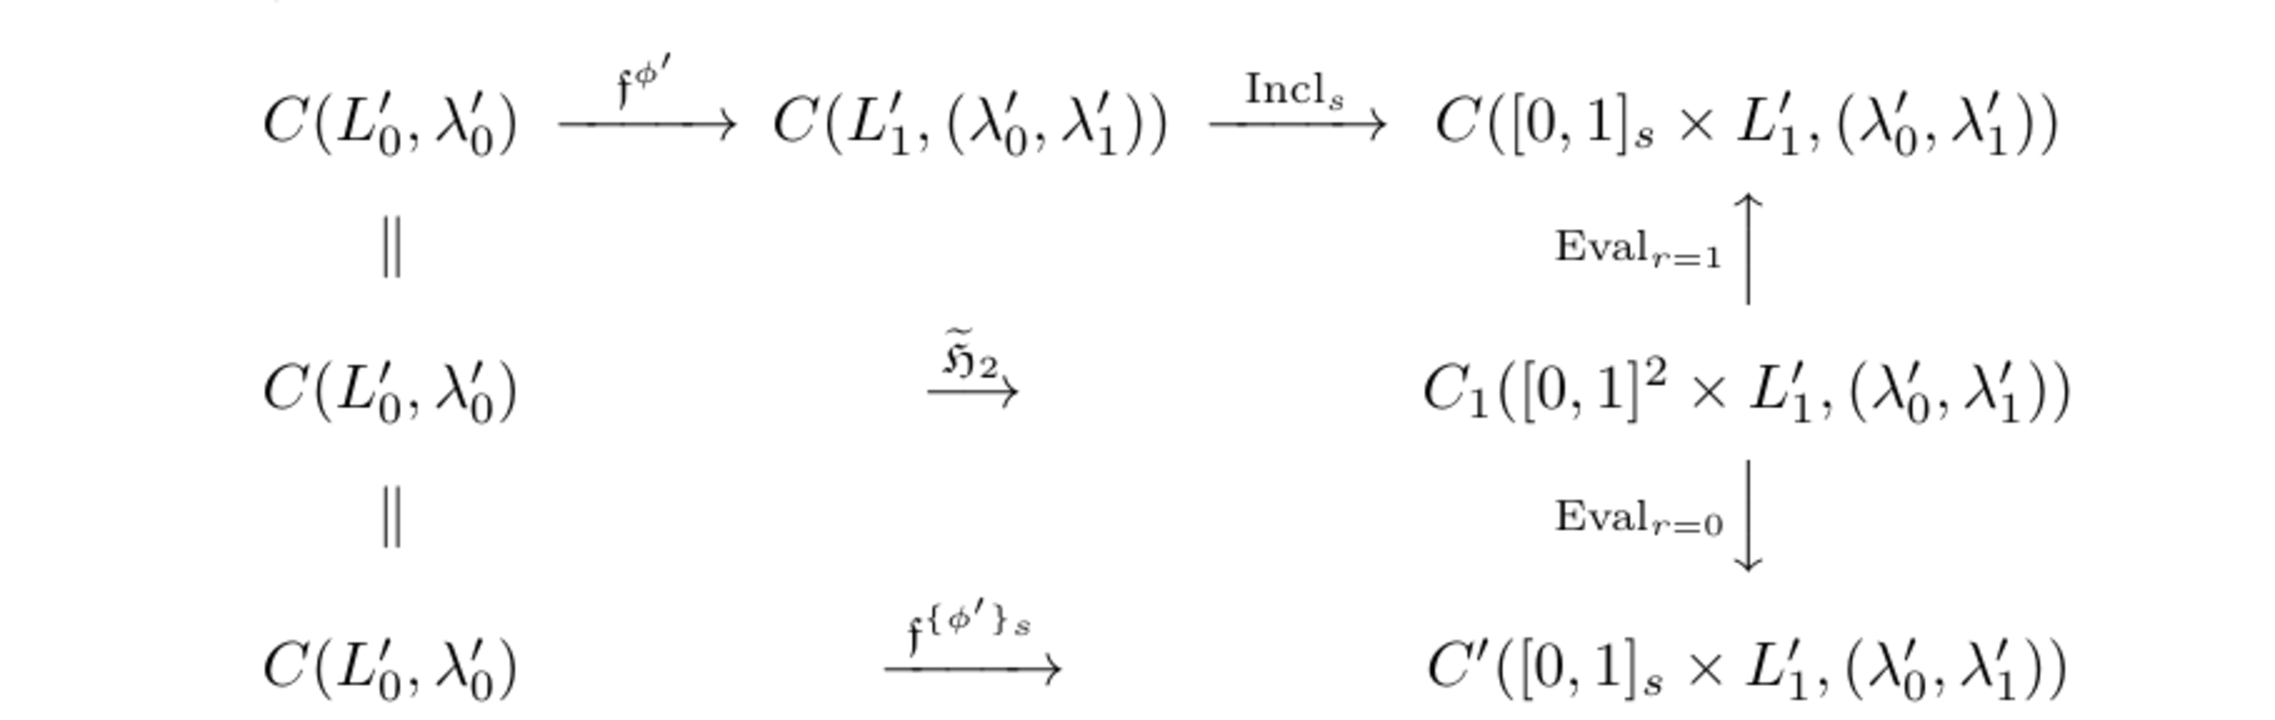
\includegraphics[width=\textwidth]{chapters/ch07-transversality/figures/phys-577-diagram-7-2-33-math-final-crop.png}
\par{\renewcommand{\thefigure}{7.2.33}\refstepcounter{figure}
\normalfont\bfseries 图式~\thefigure\label{diag:7-2-33}}
\end{minipage}\par\medskip
图式~\ref{diag:7-2-33} 中间一行的靶
保留源书标注\translatornote{图中写作 $C_1$；
但本引理刚把
$\widetilde{\mathfrak H}_2$ 的靶定义为 $C_2$，
且下文 (7.2.353) 将 $C_1$ 与 $C_2$ 胶合。
图中该处按同态型别应为 $C_2$，
此处保留原图并提示。}。
这里的
$C'([0,1]_s\times L'_1,
(\lambda'_0,\lambda'_1))$
与引理~\ref{lem:7-2-347} 中相同。
\end{lemma}

\noindent\textbf{证明。}
证明与引理~\ref{lem:7-2-347} 的证明类似
\translatornote{源书写“引理 7.2.247”，
但 7.2.247 是公式编号；
前述引理 7.2.347 才构造同类的二维模型，
此处依其定型。}，故省略。\qed

下面考虑图式~\ref{diag:7-2-34}。
由 (7.2.301.4) 可知，
该图式在子复形
$C(L'_1,\lambda'_1)\subset
C(L'_1,(\lambda'_0,\lambda'_1))$
上严格交换，因而在同伦意义下交换。
下一个引理具体给出此同伦。
令
\[
\widetilde{\mathfrak C}_3
=C([0,1]_s\times L'_1,\lambda'_1)^{[0,1]_r}.
\]
$\widetilde{\mathfrak C}_3$
是 $[0,1]^2\times C(L'_1,\lambda'_1)$
的 $A_{n',K'}$ 类模型。

\par\medskip\noindent\begin{minipage}{\textwidth}
\centering
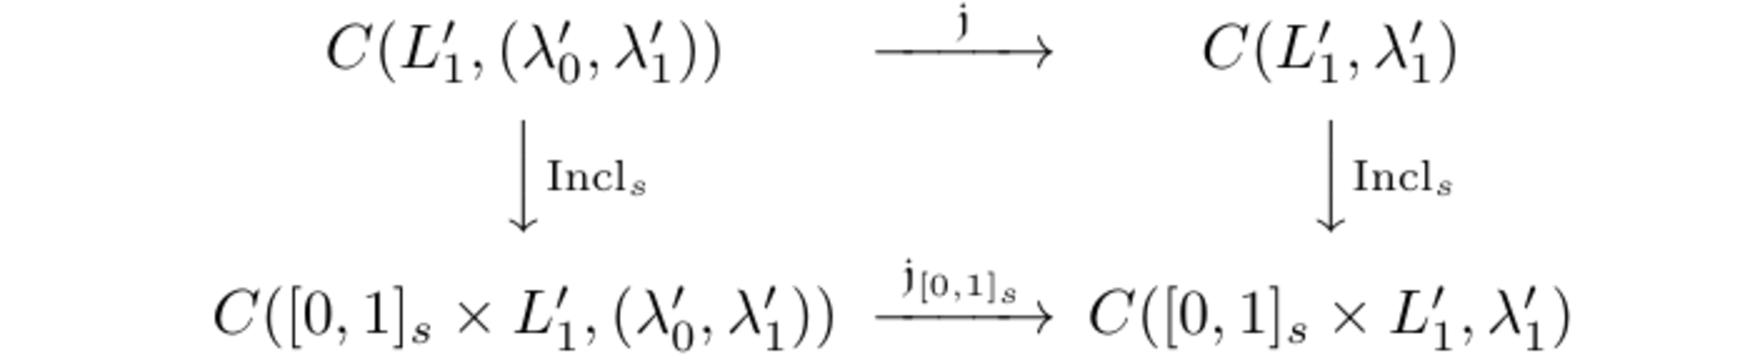
\includegraphics[width=.86\textwidth]{chapters/ch07-transversality/figures/phys-577-diagram-7-2-34-math-final-crop.png}
\par{\renewcommand{\thefigure}{7.2.34}\refstepcounter{figure}
\normalfont\bfseries 图式~\thefigure\label{diag:7-2-34}}
\end{minipage}\par\medskip

\begin{lemma}{7.2.351}\label{lem:7-2-351}
存在滤过 $A_{n',K'}$ 同态
\[
\widetilde{\mathfrak H}_3\colon
C(L'_1,(\lambda'_0,\lambda'_1))
\longrightarrow\widetilde{\mathfrak C}_3,
\]
满足下列性质：
\begin{equation}
\operatorname{Eval}_{r=0}\circ
\widetilde{\mathfrak H}_3
=j_{[0,1]_s}\circ\operatorname{Incl}_s,
\tag{7.2.352.1}\label{eq:7-2-352-1}
\end{equation}
\begin{equation}
\operatorname{Eval}_{r=1}\circ
\widetilde{\mathfrak H}_3
=\operatorname{Incl}_s\circ j,
\tag{7.2.352.2}\label{eq:7-2-352-2}
\end{equation}
\begin{equation}
\operatorname{Eval}_{s=s_0}\circ
\widetilde{\mathfrak H}_3
=\operatorname{Incl}_r\circ j.
\tag{7.2.352.3}\label{eq:7-2-352-3}
\end{equation}
\end{lemma}

\noindent\textbf{证明。}
证明是纯代数的。应用命题~\ref{prop:7-2-312}。
令
\[
C'_0=C(L'_1,\lambda'_1),\qquad
\mathfrak h\colon C(L'_1,\lambda'_1)
\longrightarrow
C(L'_1,(\lambda'_0,\lambda'_1))=C'
\]
为包含映射。
以直接的方式应用命题~\ref{prop:7-2-312}，
便得到 $\widetilde{\mathfrak H}_3$。\qed
